\subsection{Figures}
\label{rs:sec:figures}

The figures are schematic and self-contained; double lines denote colour-2
(strand) edges, single wavy lines colour-1 (cylinder) necks, and shading marks the
vertex region $\mc{V}_{0,4}$.

\begin{figure}[htp]
	\centering
	\begin{subfigure}[t]{0.48\linewidth}
		\centering
		\begin{tikzpicture}[scale=0.85, every node/.style={font=\footnotesize}]
			\foreach \y/\lab in {2/{12|34}, 0/{13|24}, -2/{14|23}} {
				\filldraw[fill=SkyBlue!25, draw=black] (-1.1,\y) circle (0.42);
				\filldraw[fill=SkyBlue!25, draw=black] (1.1,\y) circle (0.42);
				\draw[double, double distance=2pt, thick] (-0.68,\y) -- (0.68,\y);
				\draw (-1.55,\y+0.3) -- (-1.9,\y+0.55);
				\draw (-1.55,\y-0.3) -- (-1.9,\y-0.55);
				\draw (1.55,\y+0.3) -- (1.9,\y+0.55);
				\draw (1.55,\y-0.3) -- (1.9,\y-0.55);
				\node at (0,\y+0.62) {\scriptsize \lab};
			}
			\draw[-{Latex}, thick] (2.4,0) -- (3.4,0);
			\filldraw[fill=Goldenrod!45, draw=black] (4.6,0) ellipse (0.95 and 1.5);
			\node at (4.6,0) {$\mc{V}_{0,4}$};
		\end{tikzpicture}
		\caption{Three $\Sig$-exchange matchings, all mapping onto the \emph{same}
		shaded vertex region: combinatorial multiplicity $\times3$, weight
		$\tfrac13$.}
		\label{rs:fig:covering-a}
	\end{subfigure}
	\hfill
	\begin{subfigure}[t]{0.48\linewidth}
		\centering
		\begin{tikzpicture}[scale=0.85, every node/.style={font=\footnotesize}]
			\foreach \y/\lab/\col in {2/s/{Salmon}, 0/t/{PaleGreen}, -2/u/{Lavender}} {
				\filldraw[fill=gray!12, draw=black] (-1.1,\y) circle (0.42);
				\filldraw[fill=gray!12, draw=black] (1.1,\y) circle (0.42);
				\draw[thick, decorate, decoration={snake, amplitude=1.2pt, segment length=5pt}]
				(-0.68,\y) -- (0.68,\y);
				\draw (-1.55,\y+0.3) -- (-1.9,\y+0.55);
				\draw (-1.55,\y-0.3) -- (-1.9,\y-0.55);
				\draw (1.55,\y+0.3) -- (1.9,\y+0.55);
				\draw (1.55,\y-0.3) -- (1.9,\y-0.55);
				\node at (0,\y+0.55) {\scriptsize $\lab$};
				\filldraw[fill=\col!55, draw=black] (4.6,\y) ellipse (0.6 and 0.45);
				\node at (4.6,\y) {\scriptsize $\mc{M}_{\lab}$};
			}
			\draw[-{Latex}, thick] (2.4,0) -- (3.4,0);
		\end{tikzpicture}
		\caption{The $s,t,u$ cylinder channels, mapping onto \emph{disjoint}
		propagator regions: geometric tiling, $\times1$ each.}
		\label{rs:fig:covering-b}
	\end{subfigure}
	\caption{\textbf{F1.} The covering of $\mc{M}_{0,4}$
	(\cref{sec:order:amplitude}). Colour-2 (double-line) exchange is combinatorial: all
	three matchings reproduce the entire vertex region. Colour-1 (wavy cylinder)
	exchange is geometric: the three channels tile disjoint regions.}
	\label{rs:fig:covering}
\end{figure}

\begin{figure}[htp]
	\centering
	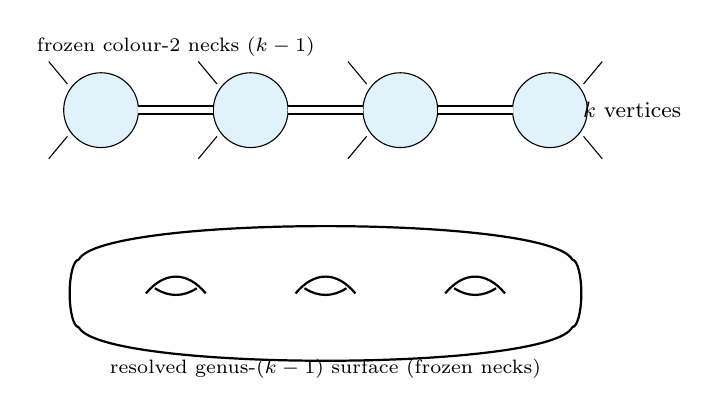
\begin{tikzpicture}[scale=0.95, every node/.style={font=\footnotesize}]
		\foreach \x in {0,2,4} {
			\filldraw[fill=SkyBlue!25, draw=black] (\x,1.3) circle (0.5);
			\draw (\x-0.45,1.65) -- (\x-0.7,1.95);
			\draw (\x-0.45,0.95) -- (\x-0.7,0.65);
		}
		\filldraw[fill=SkyBlue!25, draw=black] (6,1.3) circle (0.5);
		\draw (6+0.45,1.65) -- (6+0.7,1.95);
		\draw (6+0.45,0.95) -- (6+0.7,0.65);
		\foreach \x in {0,2,4} {
			\draw[double, double distance=2pt, thick] (\x+0.5,1.3) -- (\x+1.5,1.3);
		}
		\node at (7.1,1.3) {$k$ vertices};
		\node at (1,2.15) {\scriptsize frozen colour-2 necks ($k-1$)};
		\draw[thick] (-0.3,-0.7) .. controls (0,-0.1) and (6,-0.1) .. (6.3,-0.7);
		\draw[thick] (-0.3,-1.6) .. controls (0,-2.2) and (6,-2.2) .. (6.3,-1.6);
		\draw[thick] (-0.3,-0.7) arc (90:270:0.12 and 0.45);
		\draw[thick] (6.3,-0.7) arc (90:-90:0.12 and 0.45);
		\foreach \x in {1,3,5} {
			\draw[thick] (\x-0.4,-1.15) .. controls (\x-0.15,-0.85) and (\x+0.15,-0.85) .. (\x+0.4,-1.15);
			\draw[thick] (\x-0.28,-1.08) .. controls (\x-0.1,-1.2) and (\x+0.1,-1.2) .. (\x+0.28,-1.08);
		}
		\node at (3,-2.15) {\scriptsize resolved genus-$(k-1)$ surface (frozen necks)};
	\end{tikzpicture}
	\caption{\textbf{F2.} A length-$k$ chain of four-punctured spheres joined by
	$k-1$ frozen colour-2 necks (top), and the resolved genus-$(k-1)$ surface it
	stands for (bottom). The resolved handles are frozen and unpaid-for: the
	physical grading is that of the coloured tree (\Cref{rs:tab:grading}).}
	\label{rs:fig:chain}
\end{figure}

\begin{figure}[htp]
	\centering
	\begin{subfigure}[c]{0.48\linewidth}
		\centering
		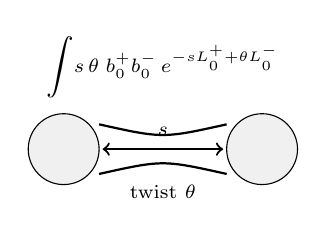
\begin{tikzpicture}[scale=0.9, every node/.style={font=\footnotesize}]
			\filldraw[fill=gray!12, draw=black] (-1.4,0) circle (0.5);
			\filldraw[fill=gray!12, draw=black] (1.4,0) circle (0.5);
			\draw[thick] (-0.9,0.35) .. controls (0,0.15) .. (0.9,0.35);
			\draw[thick] (-0.9,-0.35) .. controls (0,-0.15) .. (0.9,-0.35);
			\draw[<->, thick] (-0.85,0) -- (0.85,0);
			\node at (0,0.25) {\scriptsize $s$};
			\node at (0,-0.6) {\scriptsize twist $\theta$};
			\node at (0,1.15) {\scriptsize $\displaystyle\int\!\dd s\,\dd\theta\;b_0^+ b_0^-\,e^{-sL_0^+ + \I\theta L_0^-}$};
		\end{tikzpicture}
		\caption{Colour-1 edge \eqref{rs:eq:sewing}: a two-parameter cylinder family
		with two $b$-insertions. Geometric, propagating.}
		\label{rs:fig:kernels-a}
	\end{subfigure}
	\hfill
	\begin{subfigure}[c]{0.48\linewidth}
		\centering
		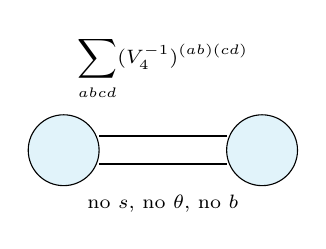
\begin{tikzpicture}[scale=0.9, every node/.style={font=\footnotesize}]
			\filldraw[fill=SkyBlue!25, draw=black] (-1.4,0) circle (0.5);
			\filldraw[fill=SkyBlue!25, draw=black] (1.4,0) circle (0.5);
			\draw[thick] (-0.9,0.2) -- (0.9,0.2);
			\draw[thick] (-0.9,-0.2) -- (0.9,-0.2);
			\node at (0,1.15) {\scriptsize $\displaystyle\sum_{abcd}(V_4^{-1})^{(ab)(cd)}$};
			\node at (0,-0.75) {\scriptsize no $s$, no $\theta$, no $b$};
		\end{tikzpicture}
		\caption{Colour-2 edge \eqref{rs:eq:c2insert}: a rigid two-strand state
		sandwich, no moduli, no $b$'s. Frozen, auxiliary.}
		\label{rs:fig:kernels-b}
	\end{subfigure}
	\caption{\textbf{F4.} The two internal kernels side by side
	(\Cref{rs:sec:kernels,rs:sec:operad}). The presence versus absence of the
	$(s,\theta)$ family and its $b$'s is the entire geometric distinction between
	propagating and auxiliary.}
	\label{rs:fig:kernels}
\end{figure}

\begin{figure}[htp]
	\centering
	\begin{tikzpicture}[scale=0.95, every node/.style={font=\footnotesize}]
		\filldraw[fill=SkyBlue!25, draw=black] (-1.7,0) ellipse (0.6 and 0.9);
		\filldraw[fill=SkyBlue!25, draw=black] (1.7,0) ellipse (0.6 and 0.9);
		\node at (-1.7,-1.25) {\scriptsize $\mc{V}_{0,6}$};
		\node at (1.7,-1.25) {\scriptsize $\mc{V}_{0,6}$};
		\foreach \y in {0.35,0,-0.35} {
			\draw[thick] (-1.1,\y) -- (1.1,\y);
		}
		\node at (0,0.95) {\scriptsize colour-3 cable ($3$ strands, $G_3^{-1}$)};
		\foreach \y in {0.5,0,-0.5} {
			\draw (-2.25,\y) -- (-2.7,\y);
			\draw (2.25,\y) -- (2.7,\y);
		}
		\draw[-{Latex}, thick] (0,-1.7) -- (0,-2.3);
		\begin{scope}[yshift=-3.4cm]
			\draw[thick] (-2.2,0.55) .. controls (-2,1.05) and (2,1.05) .. (2.2,0.55);
			\draw[thick] (-2.2,-0.55) .. controls (-2,-1.05) and (2,-1.05) .. (2.2,-0.55);
			\draw[thick] (-2.2,0.55) arc (90:270:0.12 and 0.55);
			\draw[thick] (2.2,0.55) arc (90:-90:0.12 and 0.55);
			\foreach \x in {-0.9,0.9} {
				\draw[thick] (\x-0.4,-0.05) .. controls (\x-0.15,0.28) and (\x+0.15,0.28) .. (\x+0.4,-0.05);
				\draw[thick] (\x-0.28,0.02) .. controls (\x-0.1,-0.12) and (\x+0.1,-0.12) .. (\x+0.28,0.02);
			}
			\node at (0,-0.95) {\scriptsize resolved genus-$2$ surface (frozen)};
		\end{scope}
	\end{tikzpicture}
	\caption{\textbf{F3.} A single colour-3 cable ($3$ strands, contraction
	$G_3^{-1}$) between two dressed six-punctured vertex regions, and the resolved
	genus-$2$ surface it stands for: $g_{\rm res}=k-1=2$ from \eqref{rs:eq:genus},
	physical genus $0$. See \Cref{rs:sec:tower}.}
	\label{rs:fig:cable}
\end{figure}

\begin{figure}[htp]
	\centering
	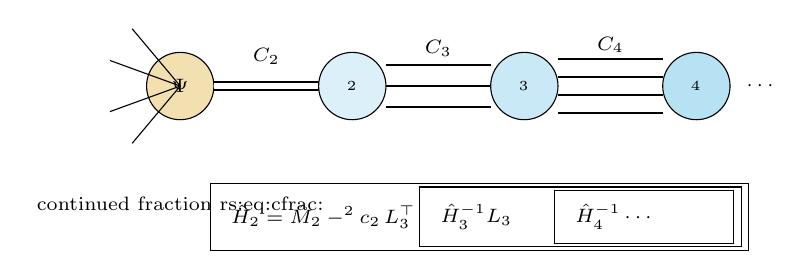
\begin{tikzpicture}[scale=0.95, every node/.style={font=\footnotesize}]
		\filldraw[fill=Goldenrod!35, draw=black] (0,0) circle (0.45);
		\node at (0,0) {\scriptsize $\Psi$};
		\foreach \a in {200,230,160,130} { \draw (0,0) -- (\a:1.0); }
		\draw[double, double distance=2pt, thick] (0.45,0) -- (1.85,0);
		\filldraw[fill=SkyBlue!30, draw=black] (2.3,0) circle (0.45);
		\node at (2.3,0) {\scriptsize $\Sig_2$};
		\node at (1.15,0.4) {\scriptsize $C_2$};
		\foreach \y in {0.28,0,-0.28} { \draw[thick] (2.75,\y) -- (4.15,\y); }
		\filldraw[fill=SkyBlue!45, draw=black] (4.6,0) circle (0.45);
		\node at (4.6,0) {\scriptsize $\Sig_3$};
		\node at (3.45,0.5) {\scriptsize $C_3$};
		\foreach \y in {0.36,0.12,-0.12,-0.36} { \draw[thick] (5.05,\y) -- (6.45,\y); }
		\filldraw[fill=SkyBlue!60, draw=black] (6.9,0) circle (0.45);
		\node at (6.9,0) {\scriptsize $\Sig_4$};
		\node at (5.75,0.55) {\scriptsize $C_4$};
		\node at (7.75,0) {\scriptsize $\cdots$};
		\begin{scope}[yshift=-2.2cm]
			\node at (0,0.6) {\scriptsize continued fraction \eqref{rs:eq:cfrac}:};
			\draw (0.4,0) rectangle (7.6,0.9);
			\node[anchor=west] at (0.55,0.45) {\scriptsize $\hat H_2=\hat M_2-\gs^2 c_2\,L_3^\top$};
			\draw (3.2,0.05) rectangle (7.5,0.85);
			\node[anchor=west] at (3.35,0.45) {\scriptsize $\hat H_3^{-1}L_3$};
			\draw (5.0,0.1) rectangle (7.4,0.8);
			\node[anchor=west] at (5.15,0.45) {\scriptsize $\hat H_4^{-1}\cdots$};
		\end{scope}
	\end{tikzpicture}
	\caption{\textbf{F5.} The scheme-B tower as a coloured tree: cables of
	increasing strand number $C_2,C_3,C_4,\dots$ (\Cref{rs:eq:colours}), with the
	continued fraction \eqref{rs:eq:cfrac} as nested boxes (each $\hat H_{k+1}^{-1}$
	sandwiched between $L_{k+1}$'s). Everything is a tree in the coloured grading;
	the nesting telescopes to contact support.}
	\label{rs:fig:tower}
\end{figure}

